\documentclass{article}
\usepackage{amsmath, amssymb, graphicx}
\usepackage{algorithm}
\usepackage{algpseudocode}
\usepackage{listings}
\usepackage{xcolor}
\lstdefinelanguage{JavaScript}{
  keywords={break, case, catch, continue, debugger, default, delete, do, else, finally, for, function, if, in, instanceof, new, return, switch, throw, try, typeof, var, void, while, with, let, const},
  keywordstyle=\color{blue}\bfseries,
  ndkeywords={class, export, boolean, throw, implements, import, this},
  ndkeywordstyle=\color{darkgray}\bfseries,
  identifierstyle=\color{black},
  sensitive=false,
  comment=[l]{//},
  morecomment=[s]{/*}{*/},
  commentstyle=\color{codegreen}\ttfamily,
  stringstyle=\color{codepurple}\ttfamily,
  morestring=[b]',
  morestring=[b]"
}

\definecolor{codegreen}{rgb}{0,0.6,0}
\definecolor{codegray}{rgb}{0.5,0.5,0.5}
\definecolor{codepurple}{rgb}{0.58,0,0.82}
\definecolor{backcolour}{rgb}{0.95,0.95,0.92}

\lstdefinestyle{mystyle}{
    backgroundcolor=\color{backcolour},   
    commentstyle=\color{codegreen},
    keywordstyle=\color{magenta},
    numberstyle=\tiny\color{codegray},
    stringstyle=\color{codepurple},
    basicstyle=\ttfamily\footnotesize,
    breakatwhitespace=false,         
    breaklines=true,                 
    captionpos=b,                    
    keepspaces=true,                 
    numbers=left,                    
    numbersep=5pt,                  
    showspaces=false,                
    showstringspaces=false,
    showtabs=false,                  
    tabsize=2
}

\lstset{style=mystyle}

\title{CS2241 Assignment 1}
\author{Nico Fidalgo}
\date{March 26, 2025}

\begin{document}

\maketitle

\section{Problem 1: PageRank and HITS Algorithm Analysis}

\subsection{Problem Statement}
We are given a directed graph represented by the following adjacency matrix.

\begin{equation}
A = 
\begin{pmatrix}
0 & 0 & 1 & 1 & 0 & 1 \\
0 & 0 & 1 & 0 & 0 & 1 \\
0 & 0 & 0 & 1 & 0 & 1 \\
0 & 1 & 1 & 0 & 0 & 0 \\
1 & 0 & 0 & 0 & 0 & 0 \\
0 & 0 & 0 & 0 & 1 & 0
\end{pmatrix}
\end{equation}

We need to calculate the PageRank scores and Hub and Authority scores. The interpretation of the adjacency matrix is:

\begin{itemize}
    \item Node $a$ has outgoing edges to nodes $c$, $d$, and $f$
    \item Node $b$ has outgoing edges to nodes $c$ and $f$
    \item Node $c$ has outgoing edges to nodes $d$ and $f$
    \item Node $d$ has outgoing edges to nodes $b$ and $c$
    \item Node $e$ has an outgoing edge to node $a$
    \item Node $f$ has an outgoing edge to node $e$
\end{itemize}

\subsection{PageRank Algorithm}
PageRank was designed to model the behavior of a random surfer on the web. The algorithm assigns a score to each node in a directed graph based on its structural importance. The intuition is that a node is important if many important nodes point to it and the importance of a node is divided among its outgoing links.

\begin{equation}
\mathbf{p} = (1-d) \cdot \frac{\mathbf{1}}{n} + d \cdot M \cdot \mathbf{p}
\end{equation}

where:
\begin{itemize}
    \item $d$ is the damping factor (typically 0.85)
    \item $n$ is the number of nodes
    \item $\mathbf{1}$ is a vector of all 1's
    \item $M$ is the transition matrix (columns sum to 1)
\end{itemize}

For each node $i$ with outgoing links, we set:
\begin{equation}
M_{j,i} = \frac{1}{\text{out-degree}(i)}
\end{equation}
if there is a link from node $i$ to node $j$, and 0 otherwise. The algorithm for computing PageRank scores is:

\begin{algorithm}
\caption{PageRank Score Calculation}
\begin{algorithmic}[1]
\State Initialize $\mathbf{p}^{(0)} = \frac{1}{n} \cdot \mathbf{1}$
\For{$t = 0, 1, 2, \ldots$ until convergence}
    \State $\mathbf{p}^{(t+1)} = (1-d) \cdot \frac{\mathbf{1}}{n} + d \cdot M \cdot \mathbf{p}^{(t)}$
    \If{$\|\mathbf{p}^{(t+1)} - \mathbf{p}^{(t)}\| < \text{tolerance}$}
        \State \textbf{break}
    \EndIf
\EndFor
\State Normalize $\mathbf{p}$ to sum to 1
\end{algorithmic}
\end{algorithm}

\subsection{PageRank Implementation}
I wrote a JavaScript program to implement the PageRank algorithm:

\begin{lstlisting}[language=JavaScript]
import * as math from 'mathjs';

// Adjacency matrix from the problem
const A = [
    [0, 0, 1, 1, 0, 1],  // a -> *
    [0, 0, 1, 0, 0, 1],  // b -> *
    [0, 0, 0, 1, 0, 1],  // c -> *
    [0, 1, 1, 0, 0, 0],  // d -> *
    [1, 0, 0, 0, 0, 0],  // e -> *
    [0, 0, 0, 0, 1, 0]   // f -> *
];

// Number of nodes
const n = A.length;

// Out-degrees
const out_degrees = A.map(row => row.reduce((sum, val) => sum + val, 0));
console.log("Out-degrees:", out_degrees);

// Create transition matrix (column-stochastic)
const M = Array(n).fill().map(() => Array(n).fill(0));
for (let i = 0; i < n; i++) {
    for (let j = 0; j < n; j++) {
        if (A[i][j] > 0) {
            M[j][i] = 1.0 / out_degrees[i];
        }
    }
}

// PageRank parameters
const d = 0.85;  // Damping factor
const max_iter = 100;
const tol = 1e-6;

// Initialize PageRank
let pr = Array(n).fill(1/n);

// Algorithm iteration
for (let iter = 0; iter < max_iter; iter++) {
    // Calculate M * pr
    const M_pr = Array(n).fill(0);
    for (let i = 0; i < n; i++) {
        for (let j = 0; j < n; j++) {
            M_pr[i] += M[i][j] * pr[j];
        }
    }
    
    // Calculate (1-d)/n + d * (M * pr)
    const pr_new = M_pr.map(val => (1-d)/n + d * val);
    
    // Check convergence
    const diff = math.norm(pr_new.map((val, idx) => val - pr[idx]));
    if (diff < tol) {
        pr = pr_new;
        console.log(`\nPageRank converged after ${iter+1} iterations.`);
        break;
    }
    
    pr = pr_new;
}

// Normalize to sum to 1
const pr_sum = pr.reduce((sum, val) => sum + val, 0);
pr = pr.map(val => val / pr_sum);
\end{lstlisting}

\subsection{PageRank Results}
After running the algorithm, I obtained the following PageRank scores:

\begin{center}
\begin{tabular}{|c|c|}
\hline
\textbf{Node} & \textbf{PageRank Score} \\
\hline
$a$ & 0.186551 \\
$b$ & 0.091079 \\
$c$ & 0.182643 \\
$d$ & 0.155479 \\
$e$ & 0.190060 \\
$f$ & 0.194188 \\
\hline
\end{tabular}
\end{center}

Nodes $f$, $e$, and $a$ have the highest PageRank scores, indicating they are structurally important in this network. Node $b$ has the lowest score, suggesting it's less central in the graph's link structure.

\subsection{HITS Algorithm}
The Hyperlink-Induced Topic Search (HITS) algorithm identifies two types of important nodes in a directed graph: hubs which are nodes that point to many good authorities, and authorities which are nodes that are pointed to by many good hubs. The hub ($\mathbf{h}$) and authority ($\mathbf{a}$) vectors satisfy:
\begin{align}
\mathbf{a} &= A^T \mathbf{h} \\
\mathbf{h} &= A \mathbf{a}
\end{align}

where $A$ is the adjacency matrix of the graph. The algorithm for computing HITS scores is:

\begin{algorithm}
\caption{HITS Score Calculation}
\begin{algorithmic}[1]
\State Initialize $\mathbf{h}^{(0)} = \mathbf{1}$ and $\mathbf{a}^{(0)} = \mathbf{1}$
\For{$t = 0, 1, 2, \ldots$ until convergence}
    \State $\mathbf{a}^{(t+1)} = A^T \mathbf{h}^{(t)}$
    \State Normalize $\mathbf{a}^{(t+1)}$
    \State $\mathbf{h}^{(t+1)} = A \mathbf{a}^{(t+1)}$
    \State Normalize $\mathbf{h}^{(t+1)}$
    \If{$\|\mathbf{a}^{(t+1)} - \mathbf{a}^{(t)}\| < \text{tolerance}$ and $\|\mathbf{h}^{(t+1)} - \mathbf{h}^{(t)}\| < \text{tolerance}$}
        \State \textbf{break}
    \EndIf
\EndFor
\end{algorithmic}
\end{algorithm}

\subsection{HITS Implementation}
Again, I wrote a JavaScript program to implement the HITS algorithm:

\begin{lstlisting}[language=JavaScript]
import * as math from 'mathjs';

// Adjacency matrix from the problem
const A = [
    [0, 0, 1, 1, 0, 1],  // a -> *
    [0, 0, 1, 0, 0, 1],  // b -> *
    [0, 0, 0, 1, 0, 1],  // c -> *
    [0, 1, 1, 0, 0, 0],  // d -> *
    [1, 0, 0, 0, 0, 0],  // e -> *
    [0, 0, 0, 0, 1, 0]   // f -> *
];

// Number of nodes
const n = A.length;

// HITS parameters
const max_iter = 100;
const tol = 1e-6;

// Initialize hub and authority scores
let hub = Array(n).fill(1);
let auth = Array(n).fill(1);

// Compute transpose of A
const AT = Array(n).fill().map(() => Array(n).fill(0));
for (let i = 0; i < n; i++) {
    for (let j = 0; j < n; j++) {
        AT[i][j] = A[j][i];
    }
}

// HITS iteration
for (let iter = 0; iter < max_iter; iter++) {
    // Update authority scores: a = A^T * h
    const auth_new = Array(n).fill(0);
    for (let i = 0; i < n; i++) {
        for (let j = 0; j < n; j++) {
            auth_new[i] += AT[i][j] * hub[j];
        }
    }
    
    // Normalize authority scores
    const auth_norm = math.norm(auth_new);
    const auth_normalized = auth_new.map(val => val / auth_norm);
    
    // Update hub scores: h = A * a
    const hub_new = Array(n).fill(0);
    for (let i = 0; i < n; i++) {
        for (let j = 0; j < n; j++) {
            hub_new[i] += A[i][j] * auth_normalized[j];
        }
    }
    
    // Normalize hub scores
    const hub_norm = math.norm(hub_new);
    const hub_normalized = hub_new.map(val => val / hub_norm);
    
    // Check convergence
    const auth_diff = math.norm(auth_normalized.map((val, idx) => val - auth[idx]));
    const hub_diff = math.norm(hub_normalized.map((val, idx) => val - hub[idx]));
    
    if (auth_diff < tol && hub_diff < tol) {
        auth = auth_normalized;
        hub = hub_normalized;
        console.log(`HITS converged after ${iter+1} iterations.`);
        break;
    }
    
    auth = auth_normalized;
    hub = hub_normalized;
}
\end{lstlisting}

\subsection{HITS Results}
After running the HITS algorithm, I obtained the following scores:

\begin{center}
\begin{tabular}{|c|c|c|}
\hline
\textbf{Node} & \textbf{Hub Score} & \textbf{Authority Score} \\
\hline
$a$ & 0.684439 & 0.000000 \\
$b$ & 0.501536 & 0.113935 \\
$c$ & 0.446890 & 0.590796 \\
$d$ & 0.283360 & 0.454889 \\
$e$ & 0.000000 & 0.000000 \\
$f$ & 0.000000 & 0.656548 \\
\hline
\end{tabular}
\end{center}

Nodes $a$, $b$, and $c$ have high hub scores, indicating they are good at pointing to authority nodes. This makes sense as $a$ and $b$ point to multiple nodes including high authority nodes $c$ and $f$. Nodes $e$ and $f$ have zero hub scores because they don't point to any nodes with high authority scores.

Nodes $f$ and $c$ have the highest authority scores, followed by node $d$. This means they are pointed to by good hub nodes. Again, this makes sense as node $f$ and $c$ are pointed to by nodes $a$ and $b$ which have high hub scores. Nodes $a$ and $e$ have zero authority scores because they aren't pointed to by any good hub nodes.

\subsection{Assumptions}
For PageRank scores:
\begin{itemize}
    \item Used a damping factor of 0.85 (standard value)
    \item Defined convergence as when L2 norm difference $< 10^{-6}$
\end{itemize}

For HITS:
\begin{itemize}
    \item Defined convergence as when L2 norm difference $< 10^{-6}$
\end{itemize}

\section{Problem 2: Random Walk Methods for Hub and Authority Scores}

\subsection{Problem Statement}
We need to prove that the Hub score for a page is proportional to the number of outlinks and that the Authority score is proportional to the number of inlinks when using the following random walk approach:


\textbf{For Authority scores:}
\begin{itemize}
    \item From page $p_1$, follow back a random inlink to page $p_2$
    \item From $p_2$, follow forward a random outlink to page $p_3$
    \item The step takes us from $p_1$ to $p_3$
\end{itemize}

\textbf{For Hub scores:}
\begin{itemize}
    \item From page $p_1$, follow forward a random outlink to page $p_2$
    \item From $p_2$, follow backward a random inlink to page $p_3$
    \item The step takes us from $p_1$ to $p_3$
\end{itemize}

We assume the Markov chains are finite, irreducible, and aperiodic, ensuring a unique stationary distribution.

\subsection{Definitions}
\begin{itemize}
    \item $A[i,j] = 1$ if there's a link from page $i$ to page $j$, 0 otherwise
    \item $\text{in}(j) = \text{number of inlinks to page } j = \sum_i A[i,j]$
    \item $\text{out}(i) = \text{number of outlinks from page } i = \sum_j A[i,j]$
\end{itemize}

\subsection{Transition Probabilities}

\textbf{For Authority Random Walk:}\\
When starting at page $i$:
\begin{itemize}
    \item The probability of following a random inlink back to page $k$ is $\frac{A[k,i]}{\text{in}(i)}$
    \item The probability of following a random outlink from $k$ to $j$ is $\frac{A[k,j]}{\text{out}(k)}$
\end{itemize}

Therefore, the transition probability from $i$ to $j$ is:
\begin{equation}
    P_a(i,j) = \sum_k \frac{A[k,i]}{\text{in}(i)} \times \frac{A[k,j]}{\text{out}(k)}
\end{equation}

\textbf{For Hub Random Walk:}\\
When starting at page $i$:
\begin{itemize}
    \item The probability of following a random outlink to page $k$ is $\frac{A[i,k]}{\text{out}(i)}$
    \item The probability of following a random inlink back from $k$ to $j$ is $\frac{A[j,k]}{\text{in}(k)}$
\end{itemize}

Therefore, the transition probability from $i$ to $j$ is:
\begin{equation}
    P_h(i,j) = \sum_k \frac{A[i,k]}{\text{out}(i)} \times \frac{A[j,k]}{\text{in}(k)}
\end{equation}

\subsection{Authority Score Proof}

Let's hypothesize that the stationary distribution $\pi_a(i)$ is proportional to $\text{in}(i)$, i.e., $\pi_a(i) = c \times \text{in}(i)$ for some constant $c$.

For this to be a stationary distribution, it must satisfy:
\begin{equation}
    \pi_a(j) = \sum_i \pi_a(i) P_a(i,j)
\end{equation}

Substituting our hypothesis:
\begin{align}
    \pi_a(j) &= \sum_i c \times \text{in}(i) \times \sum_k \frac{A[k,i]}{\text{in}(i)} \times \frac{A[k,j]}{\text{out}(k)}\\
    &= c \times \sum_i \sum_k \frac{A[k,i] \times A[k,j]}{\text{out}(k)}\\
    &= c \times \sum_k \frac{A[k,j]}{\text{out}(k)} \times \sum_i A[k,i]
\end{align}

Since $\sum_i A[k,i] = \text{out}(k)$ (the number of outlinks from page $k$):
\begin{align}
    \pi_a(j) &= c \times \sum_k \frac{A[k,j]}{\text{out}(k)} \times \text{out}(k)\\
    &= c \times \sum_k A[k,j]\\
    &= c \times \text{in}(j)
\end{align}

This confirms the hypothesis that the Authority score $\pi_a(j)$ is proportional to $\text{in}(j)$, the number of inlinks to page $j$.

\subsection{Hub Score Proof}

Similarly, hypothesize that the stationary distribution $\pi_h(i)$ is proportional to $\text{out}(i)$, i.e., $\pi_h(i) = d \times \text{out}(i)$ for some constant $d$.

For this to be a stationary distribution, it must satisfy:
\begin{equation}
    \pi_h(j) = \sum_i \pi_h(i) P_h(i,j)
\end{equation}

Substituting our hypothesis:
\begin{align}
    \pi_h(j) &= \sum_i d \times \text{out}(i) \times \sum_k \frac{A[i,k]}{\text{out}(i)} \times \frac{A[j,k]}{\text{in}(k)}\\
    &= d \times \sum_i \sum_k \frac{A[i,k] \times A[j,k]}{\text{in}(k)}\\
    &= d \times \sum_k \frac{A[j,k]}{\text{in}(k)} \times \sum_i A[i,k]
\end{align}

Since $\sum_i A[i,k] = \text{in}(k)$ (the number of inlinks to page $k$):
\begin{align}
    \pi_h(j) &= d \times \sum_k \frac{A[j,k]}{\text{in}(k)} \times \text{in}(k)\\
    &= d \times \sum_k A[j,k]\\
    &= d \times \text{out}(j)
\end{align}

This confirms the hypothesis that the Hub score $\pi_h(j)$ is proportional to $\text{out}(j)$, the number of outlinks from page $j$.

\section{Problem 3: Reservoir Sampling}

\subsection{Single-Item Reservoir Sampling}
We need to prove that the following algorithm maintains a uniform sample of one item among all items seen so far:
\begin{itemize}
    \item When the first item appears, store it in memory
    \item When the $k$-th item appears, replace the current item with probability $1/k$
\end{itemize}

I will prove by induction that after processing $k$ items, each item has exactly $1/k$ probability of being in memory. In the base case where $k=1$, after seeing the 1st item, it is stored with probability 1. Since we've only seen one item, this gives us a uniform distribution. Beyond the base case, assume that after seeing $k-1$ items, each item has a probability of $1/(k-1)$ of being in memory. Now the $k$-th item arrives. For the $k$-th item, the probability it replaces the current item is $1/k$, therefore, $P(k\text{-th item in memory}) = 1/k$. For any previous item $i$ (where $1 \leq i < k$):

\begin{align}
    P(i\text{-th item in memory after $k$ items}) &= P(i\text{-th item was in memory}) \times P(\text{it remains in memory}) \\
    &= \frac{1}{k-1} \times \left(1 - \frac{1}{k}\right) \\
    &= \frac{1}{k-1} \times \frac{k-1}{k} \\
    &= \frac{1}{k}
\end{align}

Thus, after processing the $k$-th item, each of the $k$ items seen so far has exactly $1/k$ probability of being in memory, which confirms the uniform distribution property.

\subsection{Sampling $s$ Items Without Replacement}

Now we generalize to maintaining a uniform sample of $s$ items without replacement. The algorithm is:
\begin{enumerate}
    \item Store the first $s$ items as they arrive
    \item When the $k$-th item arrives (where $k > s$):
    \begin{itemize}
        \item With probability $s/k$, include it in the sample
        \item If including it, replace a randomly chosen item from the current sample
    \end{itemize}
\end{enumerate}

I need to prove that after seeing $k$ items ($k \geq s$), each item has exactly $s/k$ probability of being in the sample. In the base case, after seeing $s$ items, all $s$ items are in the sample with probability 1. Since $s/s = 1$, this is uniform. Beyond the base case, assume that after seeing $k-1$ items ($k-1 \geq s$), each has probability $s/(k-1)$ of being in the sample. Now the $k$-th item arrives. We need to show that after processing it, each of the $k$ items has probability exactly $s/k$ of being in the sample. For the $k$-th item, it's included with probability $s/k$, so $P(k\text{-th item in sample}) = s/k$. For any previous item $i$ (where $1 \leq i < k$):

\begin{align}
    P(i\text{-th item remains in sample}) &= P(i\text{-th item was in sample}) \nonumber\\
    &\quad \times P(i\text{'s not replaced}) \\
    &= \frac{s}{k-1} \times \left[1 - P(k\text{-th item is chosen}) \right. \nonumber\\
    &\quad \left. \times P(\text{item $i$ is replaced} \mid k\text{-th is chosen})\right] \\
    &= \frac{s}{k-1} \times \left[1 - \frac{s}{k} \times \frac{1}{s}\right] \\
    &= \frac{s}{k-1} \times \left[1 - \frac{1}{k}\right] \\
    &= \frac{s}{k-1} \times \frac{k-1}{k} \\
    &= \frac{s}{k}
\end{align}

This confirms that after processing the $k$-th item, each of the $k$ items has probability $s/k$ of being in the sample, maintaining uniformity.

\subsection{Implementation}

To verify these theoretical results, I implemented both algorithms in JavaScript and ran simulations to check if the sampling is uniform.

\begin{lstlisting}[language=JavaScript]
// Single-item reservoir sampling
function singleItemReservoirSampling(stream) {
    let sample = null;
    let count = 0;
    
    for (const item of stream) {
        count++;
        if (count === 1) {
            sample = item;
        } else {
            // Replace with probability 1/count
            if (Math.random() < 1/count) {
                sample = item;
            }
        }
    }
    
    return sample;
}

// Reservoir sampling of s items without replacement
function reservoirSampling(stream, s) {
    let sample = [];
    let count = 0;
    
    for (const item of stream) {
        count++;
        
        if (count <= s) {
            // Fill the reservoir with the first s items
            sample.push(item);
        } else {
            // Decide whether to include this item in the sample
            const j = Math.floor(Math.random() * count);
            if (j < s) {
                // Replace the randomly chosen item
                sample[j] = item;
            }
        }
    }
    
    return sample;
}

// Function to simulate multiple runs and track results
function runSimulations(numRuns, streamSize, sampleSize = 1) {
    const counts = {};
    
    // Initialize counts for each number
    for (let i = 1; i <= streamSize; i++) {
        counts[i] = 0;
    }
    
    for (let run = 0; run < numRuns; run++) {
        // Create a stream of numbers from 1 to streamSize
        const stream = Array.from({length: streamSize}, (_, i) => i + 1);
        
        let result;
        if (sampleSize === 1) {
            result = [singleItemReservoirSampling(stream)];
        } else {
            result = reservoirSampling(stream, sampleSize);
        }
        
        // Update counts
        result.forEach(item => {
            counts[item]++;
        });
    }
    
    // Convert to frequencies
    const frequencies = {};
    for (const [key, value] of Object.entries(counts)) {
        frequencies[key] = value / numRuns;
    }
    
    return frequencies;
}
\end{lstlisting}

\subsection{Results}

I ran 10,000 simulations with a stream of 10 items for both single-item sampling and sampling 3 items without replacement. The results confirm our theoretical analysis:

\begin{figure}[h]
    \centering
    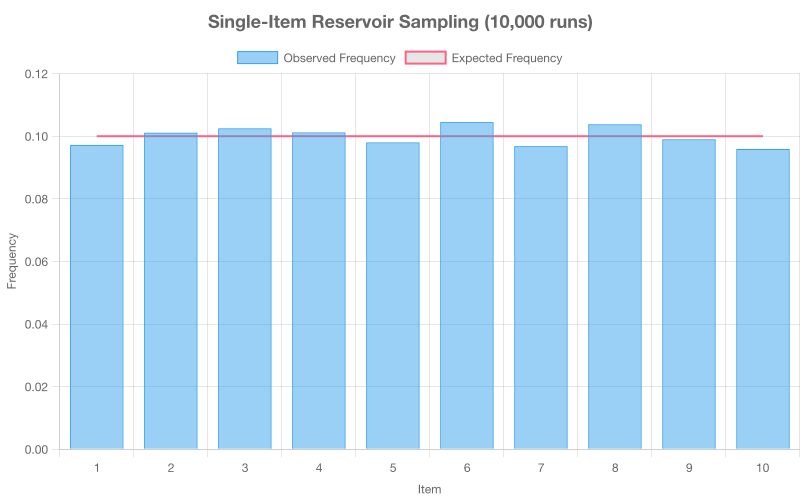
\includegraphics[width=0.8\textwidth]{images/single_item_sampling.png}
    \caption{Frequency distribution of single-item reservoir sampling over 10,000 runs. Each item has approximately 0.1 probability of being selected, as expected.}
    \label{fig:single-item-sampling}
\end{figure}

\begin{figure}[H]
    \centering
    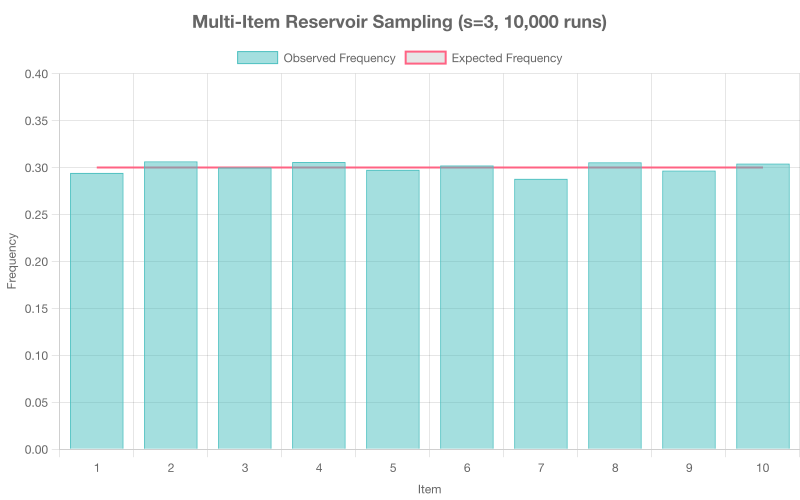
\includegraphics[width=0.8\textwidth]{images/multi_item_sampling.png}
    \caption{Frequency distribution of 3-item reservoir sampling over 10,000 runs. Each item has approximately 0.3 probability of being selected, as expected.}
    \label{fig:multi-item-sampling}
\end{figure}

For the single-item sampling, the expected frequency is $1/10 = 0.1$ for each item. The empirical results in Figure \ref{fig:single-item-sampling} closely match this expectation, with minimal deviation from the expected value. For the 3-item sampling, the expected frequency is $3/10 = 0.3$ for each item. Again, the empirical results in Figure \ref{fig:multi-item-sampling} closely match the expectation, confirming our theoretical analysis. These simulations confirm the theoretical correctness of both algorithms, showing that they indeed maintain uniform sampling of the stream at each step.

\subsection{Why This Is Useful in Streaming Algorithms}

Reservoir sampling is particularly valuable in streaming algorithms because it maintains a representative sample without needing knowledge of the total stream size, it uses constant memory as it stores only $s$ items, it processes each item in constant time, and the sample remains uniform at each step of the process. This makes it ideal for applications like processing large data streams that don't fit in memory, online analytics where a representative sample is needed in real time, distributed systems where data is generated across multiple sources, and monitoring high-volume log data where sampling is necessary for performance.

\section{Problem 4: Flipping a Coin Until First Head}

\subsection{Problem Statement}
A fair coin is flipped until the first head occurs. Let $X$ be the number of flips required. I must first find the entropy $H(X)$ in bits and then describe how to ask yes/no questions to determine $X$ adn find the expected number of such questions and compare this result to $H(X)$.

\subsection{Entropy Calculation}

Since the coin is fair, the probability that $X = k$ (i.e., the first head occurs on the $k$-th flip) is
\[
P(X = k) \;=\; \left(\frac12\right)^k,
\quad k = 1,2,3,\ldots
\]
We use the fact that for a geometric random variable with parameter $p=\tfrac12$ (counting the number of trials up to and including the first success), the distribution is:
\[
P(X = k) = \frac12 \left(\frac12\right)^{\,k-1} = \left(\frac12\right)^k.
\]
The entropy in bits is
\[
H(X) \;=\; - \sum_{k=1}^{\infty} P(X=k)\,\log_2 \bigl[P(X=k)\bigr].
\]
Substitute $P(X=k) = (1/2)^k$, and note that $\log_2 \bigl[ (1/2)^k \bigr] = -k$. So
\[
H(X)
= - \sum_{k=1}^{\infty} \left(\frac12\right)^k \bigl(-k\bigr)
= \sum_{k=1}^{\infty} k \,\left(\frac12\right)^k.
\]
We now use the series identity:
\[
\sum_{k=1}^{\infty} k \,x^k \;=\; \frac{x}{(1-x)^2}, 
\quad \text{for } -1 < x < 1.
\]
With $x = \tfrac12$, we get
\[
\sum_{k=1}^{\infty} k \left(\frac12\right)^k
= \frac{\tfrac12}{(1 - \tfrac12)^2} \;=\; \frac{\tfrac12}{(\tfrac12)^2} 
= \frac{\tfrac12}{\tfrac14} 
= 2.
\]
Thus, the entropy $H(X) = 2$ bits.

\subsection{Yes/No Questions and Comparison}

To determine $X$ from yes/no questions, we want a strategy that minimizes the expected number of questions. We can think of this as constructing a decision tree for the geometric distribution.

One possible line of reasoning is:
\begin{itemize}
    \item First question: ``Is $X=1$?'' 
        \begin{itemize}
        \item With probability $1/2$, the answer is yes, and we are done with just 1 question.
        \item With probability $1/2$, the answer is no, in which case we continue to ask about $X=2$, $X=3$, etc.
        \end{itemize}
    \item We can create a decision tree that accounts for the probabilities $(1/2)^k$ at each branch.
\end{itemize}
This geometric distribution achieves an expected number of questions exactly $2$, matching the entropy $H(X) = 2$ bits. In other words, on average, we need 2 yes/no questions to determine $X$. This matches the lower bound given by $H(X)$, illustrating that our questioning strategy is asymptotically optimal.

Hence, the entropy $H(X)$ provides a fundamental limit on the average number of bits (yes/no questions) required, and our constructed question strategy can match that limit.

\section{Problem 5: Arithmetic Coding}

\subsection{Problem Statement} 
Consider arithmetic coding for the string \texttt{abcbaab} given the probabilities:
\[
P(a)=0.2,\quad P(b)=0.3,\quad P(c)=0.5.
\]
We must (1) show each step of idealized arithmetic coding (with real-number arithmetic) for the string \texttt{abcbaab}, and then (2) decode a sequence of length 10 for the real number $0.63215699$ using the same model and intervals.

\subsection{Encoding \texttt{abcbaab}}

We begin with the interval $[0,1)$. At each step:
\[
\text{If our current interval is } [L, R),
\]
we subdivide it into subintervals based on the probabilities $0.2, 0.3,$ and $0.5$ for $a, b, c$:
\[
\begin{aligned}
&\text{Interval for } a : [\,L,\; L + 0.2(R-L)\!),\\
&\text{Interval for } b : [\,L + 0.2(R-L),\; L + 0.5(R-L)\!),\\
&\text{Interval for } c : [\,L + 0.5(R-L),\; R\!).
\end{aligned}
\]
We pick the subinterval matching the next character and let that become our new $[L,R)$.

\paragraph{String: \texttt{abcbaab}}

\begin{enumerate}
    \item \textbf{Step 1 (encode `a`):} 
    \[
    [L,R) = [0,1) \;\;\to\; 
      \text{subinterval for $a$} = [0,\,0.2).
    \]
    New interval: $[0,\,0.2)$.

    \item \textbf{Step 2 (encode `b`):}
    \[
    [L,R) = [0,\,0.2)\quad \Delta = 0.2.
    \]
    Subinterval for $b$ is $[\,L + 0.2\Delta,\; L + 0.5\Delta) = [0.04,\; 0.1).$
    New interval: $[0.04,\,0.1)$.

    \item \textbf{Step 3 (encode `c`):}
    \[
    [L,R) = [0.04,\,0.1)\quad \Delta = 0.06.
    \]
    Subinterval for $c$ is $[\,0.04 + 0.5\cdot 0.06,\; 0.1) = [0.07,\; 0.1).$
    New interval: $[0.07,\,0.1)$.

    \item \textbf{Step 4 (encode `b`):}
    \[
    [L,R) = [0.07,\,0.1)\quad \Delta = 0.03.
    \]
    Subinterval for $b$ is $[\,0.07 + 0.2\cdot 0.03,\; 0.07 + 0.5\cdot 0.03) = [0.076,\; 0.0855).$
    New interval: $[0.076,\,0.0855)$.

    \item \textbf{Step 5 (encode `a`):}
    \[
    [L,R) = [0.076,\,0.0855)\quad \Delta = 0.0095.
    \]
    Subinterval for $a$ is $[\,0.076,\; 0.076 + 0.2\cdot 0.0095) = [0.076,\; 0.0779).$
    New interval: $[0.076,\,0.0779)$.

    \item \textbf{Step 6 (encode `a`):}
    \[
    [L,R) = [0.076,\,0.0779)\quad \Delta = 0.0019.
    \]
    Subinterval for $a$ is $[\,0.076,\; 0.076 + 0.2\cdot 0.0019) = [0.076,\; 0.07638).$
    New interval: $[0.076,\,0.07638)$.

    \item \textbf{Step 7 (encode `b`):}
    \[
    [L,R) = [0.076,\,0.07638)\quad \Delta = 0.00038.
    \]
    Subinterval for $b$ is $[\,0.076 + 0.2\cdot 0.00038,\; 0.076 + 0.5\cdot 0.00038) = [0.076076,\; 0.07619)$.
    Final interval: $[0.076076,\,0.07619)$.
\end{enumerate}

Hence, the arithmetic-coded value for \texttt{abcbaab} is any real number in 
\[
[\,0.076076,\; 0.07619).
\]

\subsection{Decoding From $0.63215699$ for 10 Symbols}

We now decode a 10-symbol sequence assuming $P(a)=0.2, P(b)=0.3, P(c)=0.5$. At each step, we split the current interval $[L,R)$ into subintervals for $a, b, c$ and see where $0.63215699$ falls.

\begin{enumerate}
\item \textbf{Step 1:} Start $[0,1)$.  
  \[
    a:[0,0.2),\quad b:[0.2,0.5),\quad c:[0.5,1).
  \]
  Since $0.63215699 \in [0.5,1)$, the first symbol is $c$. 
  New interval: $[0.5,1)$.

\item \textbf{Step 2:} Interval $[0.5,1)$ (length $0.5$).  
  \[
    a:[0.5,0.6),\quad b:[0.6,0.75),\quad c:[0.75,1).
  \]
  $0.63215699 \in [0.6,0.75)\implies$ second symbol is $b$.  
  New interval: $[0.6,0.75)$.

\item \textbf{Step 3:} Interval $[0.6,0.75)$ (length $0.15$).  
  \[
    a:[0.6,0.63),\quad b:[0.63,0.675),\quad c:[0.675,0.75).
  \]
  $0.63215699 \in [0.63,0.675)\implies$ third symbol is $b$.  
  New interval: $[0.63,0.675)$.

\item \textbf{Step 4:} Interval $[0.63,0.675)$ (length $0.045$).  
  \[
    a:[0.63,0.639),\quad b:[0.639,0.6525),\quad c:[0.6525,0.675).
  \]
  $0.63215699 < 0.639\implies$ fourth symbol is $a$.  
  New interval: $[0.63,0.639)$.

\item \textbf{Step 5:} Interval $[0.63,0.639)$ (length $0.009$).  
  \[
    a:[0.63,0.6318),\quad b:[0.6318,0.6345),\quad c:[0.6345,0.639).
  \]
  $0.63215699 \in [0.6318,0.6345)\implies$ fifth symbol is $b$.  
  New interval: $[0.6318,0.6345)$.

\item \textbf{Step 6:} Interval $[0.6318,0.6345)$ (length $0.0027$).  
  \[
    a:[0.6318,0.63234),\quad b:[0.63234,0.63315),\quad c:[0.63315,0.6345).
  \]
  $0.63215699 < 0.63234\implies$ sixth symbol is $a$.  
  New interval: $[0.6318,0.63234)$.

\item \textbf{Step 7:} Interval $[0.6318,0.63234)$ (length $0.00054$).  
  \[
    a:[0.6318,0.631908),\quad b:[0.631908,0.63207),\quad c:[0.63207,0.63234).
  \]
  $0.63215699 > 0.63207\implies$ seventh symbol is $c$.  
  New interval: $[0.63207,0.63234)$.

\item \textbf{Step 8:} Interval $[0.63207,0.63234)$ (length $0.00027$).  
  \[
    a:[0.63207,0.632124),\quad b:[0.632124,0.632205),\quad c:[0.632205,0.63234).
  \]
  $0.63215699 \in [0.632124,0.632205)\implies$ eighth symbol is $b$.  
  New interval: $[0.632124,0.632205)$.

\item \textbf{Step 9:} Interval $[0.632124,0.632205)$ (length $0.000081$).  
  \[
    a:[0.632124,0.6321402),\quad b:[0.6321402,0.6321645),\quad c:[0.6321645,0.632205).
  \]
  $0.63215699 < 0.6321645\implies$ ninth symbol is $b$.  
  New interval: $[0.6321402,0.6321645)$.

\item \textbf{Step 10:} Interval $[0.6321402,0.6321645)$ (length $0.0000243$).  
  \[
    a:[0.6321402,0.63214506),\quad b:[0.63214506,0.63215235),\quad c:[0.63215235,0.6321645).
  \]
  $0.63215699 \in [0.63215235,0.6321645)\implies$ tenth symbol is $c$.
\end{enumerate}

Hence, the decoded 10-symbol sequence is
\[
c,\; b,\; b,\; a,\; b,\; a,\; c,\; b,\; b,\; c.
\]

\section{Problem 6: Compression Methods}

\subsection{Problem Statement}
We want to compress the string:
\[
\texttt{"abracadabraarbadacarba"}
\]
using three methods:
\begin{itemize}
  \item LZ77 with a window size of 6 and a lookahead buffer of size 6.
  \item LZ78.
  \item LZW (with \{\texttt{a},\texttt{b},\texttt{c},\texttt{d},\texttt{r}\} in the dictionary initially, in alphabetical order).
\end{itemize}

\subsection{LZ77 (Window = 6, Lookahead Buffer = 6)}

We scan the string \texttt{"abracadabraarbadacarba"} from left to right, always allowing up to 6 characters of search history and up to 6 characters of lookahead. We output triples $(\mathrm{distance}, \mathrm{length}, \mathrm{nextChar})$ each time. The string, indexed from 0 to 21, is:

\[
\begin{array}{l}
\text{Indices: }0\;\;1\;\;2\;\;3\;\;4\;\;5\;\;6\;\;7\;\;8\;\;9\;\;10\;11\;12\;13\;14\;15\;16\;17\;18\;19\;20\;21\\
\text{Chars:  }a\;\;b\;\;r\;\;a\;\;c\;\;a\;\;d\;\;a\;\;b\;\;r\;\;a\;\;a\;\;r\;\;b\;\;a\;\;d\;\;a\;\;c\;\;a\;\;r\;\;b\;\;a
\end{array}
\]

We encode as follows:

\begin{enumerate}
  \item \textbf{Position 0}, no search window: no match. Output $(0,0,\texttt{a})$. Move to index 1.
  \item \textbf{Position 1}, search window = `a`: no match for `b`. Output $(0,0,\texttt{b})$. Move to index 2.
  \item \textbf{Position 2}, search = `ab`: no match for `r`. Output $(0,0,\texttt{r})$. Move to index 3.
  \item \textbf{Position 3}, search = `abr`: next is `a`; we find a 1-length match for `a` (found at index 0). Next char after that is `c` (index 4). Output $(3,1,\texttt{c})$. We skip the `a` (index 3) plus that next char (index 4), so jump to index 5.
  \item \textbf{Position 5}, search (up to length 6) = `abrac` (indices 0--4). The substring `a` at index 5 matches `a` in the window (e.g., at index 3). Next char is `d` (index 6). Output $(2,1,\texttt{d})$. Move to index 7.
  \item \textbf{Position 7}, search = `bracad` (indices 1--6). The substring `a` at index 7 matches the `a` in the window (e.g., index 5). Next char is `b` (index 8). Output $(2,1,\texttt{b})$. Move to index 9.
  \item \textbf{Position 9}, search = `acadab` (indices 3--8). We see `r` at index 9 has no direct multi-length match. Output $(0,0,\texttt{r})$. Move to index 10.
  \item \textbf{Position 10}, search = `cadabr` (indices 4--9). We see `a` at index 10 can match single `a` in the window. Next char is `a` (index 11). So output $(1,1,\texttt{a})$. Move to index 12.
  \item \textbf{Position 12}, search = `dabra a` (indices 6--11). Next substring is `r` at index 12. We match `r` from index 9, length 1. Next char is `b` (index 13). Output $(3,1,\texttt{b})$. Move to index 14.
  \item \textbf{Position 14}, search = `abraar` (indices 8--13). The substring `a` at index 14 matches in the window. Next char is `d` (15). Output $(3,1,\texttt{d})$. Move to index 16.
  \item \textbf{Position 16}, search = `raarba` (indices 10--15). The substring `a` at index 16 matches the `a` at index 14. Next char is `c` (17). Output $(2,1,\texttt{c})$. Move to index 18.
  \item \textbf{Position 18}, search = `arbad a c` (indices 12--17; effectively up to 6 chars). We see `a` at 18 matches the `a` at 16. Next char is `r` (19). Output $(2,1,\texttt{r})$. Move to index 20.
  \item \textbf{Position 20}, search = `badacar` (indices 14--19). `b` at 20 is new. Output $(0,0,\texttt{b})$. Move to index 21.
  \item \textbf{Position 21}, search = `adacarb` (indices 15--20). The last character is `a`. No multi-length match; output $(0,0,\texttt{a})$. Done.
\end{enumerate}

Thus, the final sequence of LZ77 triples is:
\[
\begin{aligned}
&(0,0,\texttt{a}),\;(0,0,\texttt{b}),\;(0,0,\texttt{r}),\;(3,1,\texttt{c}),\;(2,1,\texttt{d}),\;(2,1,\texttt{b}),\\
&(0,0,\texttt{r}),\;(1,1,\texttt{a}),\;(3,1,\texttt{b}),\;(3,1,\texttt{d}),\;(2,1,\texttt{c}),\;(2,1,\texttt{r}),\\
&(0,0,\texttt{b}),\;(0,0,\texttt{a}).
\end{aligned}
\]

\subsection{LZ78}

For LZ78, we maintain a dictionary of substrings (each with an index). We scan from left to right, always outputting $(\mathrm{index}, \mathrm{nextChar})$ where index is the dictionary index of hte longest matching prefix found and nextChar is the next new character that extends that prefix.We then add that new substring (prefix + new character) to the dictionary.

\begin{enumerate}
\item Read `a` (index 0). Not in dictionary, so output $(0,\texttt{a})$. Dictionary: (1) `a`.
\item Read `b` (index 1). Not in dictionary, output $(0,\texttt{b})$. Dictionary: (1) `a`, (2) `b`.
\item Read `r` (index 2). Not in dictionary, output $(0,\texttt{r})$. Dictionary: (1) `a`, (2) `b`, (3) `r`.
\item Read `a` (index 3). That is in dictionary entry 1. Next char is `c` (index 4). Substring `ac` not in dictionary. Output $(1,\texttt{c})$. Dictionary: (1) `a`, (2) `b`, (3) `r`, (4) `ac`.
\item Now we move past `a,c` (indices 3,4). Next index 5 is `a`. That is dictionary entry 1. Next char is `d` (6). `ad` not in dictionary, so output $(1,\texttt{d})$. 
  Dictionary: (5) `ad` added.
\item Move past `a,d`. Next index 7 is `a`. That is entry 1. Next char is `b` (8). `ab` not in dictionary. Output $(1,\texttt{b})$. Dictionary: (6) `ab`.
\item Next index 9 is `r` (dictionary entry 3). Next char is `a` (10). `ra` not in dictionary. Output $(3,\texttt{a})$. Dictionary: (7) `ra`.
\item Next index 11 is `a` (entry 1). Next char is `r` (12). `ar` not in dictionary. Output $(1,\texttt{r})$. Dictionary: (8) `ar`.
\item Next index 13 is `b` (entry 2). Next char is `a` (14). `ba` not in dictionary. Output $(2,\texttt{a})$. Dictionary: (9) `ba`.
\item Index 15 is `d`. Not in dictionary, so output $(0,\texttt{d})$. Dictionary: (10) `d`.
\item Index 16 is `a` (entry 1). Next char is `c` (17). `ac` is entry 4, so we have a prefix. Then the next char after that is `a` (18): `aca` not in dictionary. So we output $(4,\texttt{a})$. Dictionary: (11) `aca`.
\item Index 19 is `r` (entry 3). Next char is `b` (20). `rb` not in dictionary. Output $(3,\texttt{b})$. Dictionary: (12) `rb`.
\item Final index 21 is `a` (entry 1), but we have no next character left. Often we do $(1,\textit{EOF})$ or a special marker. For simplicity, we can just treat it as $(0,\texttt{a})$ if we prefer a fresh literal. Here, let's do $(0,\texttt{a})$. Dictionary: (13) `a` (repeated, though duplicates can happen in LZ78).
\end{enumerate}

Therefore, the final LZ78 output pairs are:
\[
\begin{aligned}
&(0,\texttt{a}),\, (0,\texttt{b}),\, (0,\texttt{r}),\, (1,\texttt{c}),\, (1,\texttt{d}),\, (1,\texttt{b}),\\
&(3,\texttt{a}),\, (1,\texttt{r}),\, (2,\texttt{a}),\, (0,\texttt{d}),\, (4,\texttt{a}),\, (3,\texttt{b}),\, (0,\texttt{a}).
\end{aligned}
\]

\subsection{LZW}

Here, we initialize the dictionary with single characters:
\[
1=\texttt{a},\quad 2=\texttt{b},\quad 3=\texttt{c},\quad 4=\texttt{d},\quad 5=\texttt{r}.
\]
We parse the string \texttt{abracadabraarbadacarba} from left to right, building the code sequence. Let $w$ be the current working prefix.

\begin{enumerate}
\item Start $w=\varepsilon$ (empty).
\item Read `a`. $w+\texttt{a}=\texttt{a}$ is in the dictionary (code=1). Keep going.
\item Next char `b`. Now $w+\texttt{b}=\texttt{ab}$ is \emph{not} in the dictionary.  
  Output the code for $w=\texttt{a}$: that is 1.  
  Add `ab` to dictionary with a new code: $6=\texttt{ab}$.  
  Set $w=\texttt{b}$.
\item Next char `r`. $w+\texttt{r}=\texttt{br}$ is not in dictionary.  
  Output code of $w=\texttt{b}$: 2.  
  Add `br` to dictionary: $7=\texttt{br}$.  
  $w=\texttt{r}$.
\item Next char `a`. $w+\texttt{a}=\texttt{ra}$ is not in dictionary.  
  Output code of $w=\texttt{r}$: 5.  
  Add `ra`: $8=\texttt{ra}$.  
  $w=\texttt{a}$.
\item Next char `c`. $w+\texttt{c}=\texttt{ac}$ not in dictionary.  
  Output code of $w=\texttt{a}$: 1.  
  Add `ac`: $9=\texttt{ac}$.  
  $w=\texttt{c}$.
\item Next char `a`. $w+\texttt{a}=\texttt{ca}$ not in dictionary.  
  Output code of $w=\texttt{c}$: 3.  
  Add `ca`: $10=\texttt{ca}$.  
  $w=\texttt{a}$.
\item Next char `d`. $w+\texttt{d}=\texttt{ad}$ not in dictionary.  
  Output code of $w=\texttt{a}$: 1.  
  Add `ad`: $11=\texttt{ad}$.  
  $w=\texttt{d}$.
\item Next char `a`. $w+\texttt{a}=\texttt{da}$ not in dictionary.  
  Output $w=\texttt{d}$: code=4.  
  Add `da`: $12=\texttt{da}$.  
  $w=\texttt{a}$.
\item Next char `b`. $w+\texttt{b}=\texttt{ab}$ \textit{is} dictionary entry 6. So $w=\texttt{ab}$.  
  Next char `r`. $w+\texttt{r}=\texttt{abr}$ not in dictionary.  
  Output code of $w=\texttt{ab}$: 6.  
  Add `abr`: $13=\texttt{abr}$.  
  $w=\texttt{r}$.
\item Next char `a`. $w+\texttt{a}=\texttt{ra}$ is dictionary entry 8, so $w=\texttt{ra}$.  
  Next char `a`. $w+\texttt{a}=\texttt{raa}$ not in dictionary.  
  Output code($\texttt{ra}$)=8.  
  Add `raa`: $14=\texttt{raa}$.  
  $w=\texttt{a}$.
\item Next char `r`. $w+\texttt{r}=\texttt{ar}$ not in dictionary (we have `ac`, `ad`, but not `ar`).  
  Output code($\texttt{a}$)=1.  
  Add `ar`: $15=\texttt{ar}$.  
  $w=\texttt{r}$.
\item Next char `b`. $w+\texttt{b}=\texttt{rb}$ not in dictionary.  
  Output code($\texttt{r}$)=5.  
  Add `rb`: $16=\texttt{rb}$.  
  $w=\texttt{b}$.
\item Next char `a`. $w+\texttt{a}=\texttt{ba}$ not in dictionary.  
  Output code($\texttt{b}$)=2.  
  Add `ba`: $17=\texttt{ba}$.  
  $w=\texttt{a}$.
\item Next char `d`. $w+\texttt{d}=\texttt{ad}$ is dictionary entry 11, so $w=\texttt{ad}$.  
  Next char `a`. $w+\texttt{a}=\texttt{ada}$ not in dictionary.  
  Output code($\texttt{ad}$)=11.  
  Add `ada`: $18=\texttt{ada}$.  
  $w=\texttt{a}$.
\item Next char `c`. $w+\texttt{c}=\texttt{ac}$ is entry 9, so $w=\texttt{ac}$.  
  Next char `a`. $w+\texttt{a}=\texttt{aca}$ not in dictionary.  
  Output code($\texttt{ac}$)=9.  
  Add `aca`: $19=\texttt{aca}$.  
  $w=\texttt{a}$.
\item Next char `r`. $w+\texttt{r}=\texttt{ar}$ is entry 15, so $w=\texttt{ar}$.  
  Next char `b`. $w+\texttt{b}=\texttt{arb}$ not in dictionary.  
  Output code($\texttt{ar}$)=15.  
  Add `arb`: $20=\texttt{arb}$.  
  $w=\texttt{b}$.
\item Final char `a`. $w+\texttt{a}=\texttt{ba}$ is entry 17, so $w=\texttt{ba}$.  
  String ends, so output code($\texttt{ba}$)=17.
\end{enumerate}

Hence the final LZW code stream is:
\[
1,\;2,\;5,\;1,\;3,\;1,\;4,\;6,\;8,\;1,\;5,\;2,\;11,\;9,\;15,\;17
\]

\section{Problem 7: Randomized Hadamard Transform}

\subsection{Problem Statement}
Let $d=1024$. We:
\begin{enumerate}
    \item Generate a random point on the $d$-dimensional unit sphere.
    \item Rotate it using a Randomized Hadamard Transform (RHT).
    \item Quantize coordinates to $\pm 1$ by sign.
    \item Invert the transform.
    \item Measure mean squared error (MSE) vs.\ the original.
    \item Repeat 100 times. Give min, mean, max MSE.
\end{enumerate}

\subsection{Solution and Example Code}

Below is a Python script doing exactly that. It uses NumPy for the Fast Walsh-Hadamard Transform (FWHT) and random number generation. Then it prints the min/mean/max MSE from 100 trials.

\begin{verbatim}
import numpy as np

def fast_walsh_hadamard_transform(x):
    """
    In-place Fast Walsh-Hadamard Transform of x (length must be a power of 2).
    """
    n = len(x)
    h = 1
    while h < n:
        for i in range(0, n, h*2):
            for j in range(i, i+h):
                a = x[j]
                b = x[j+h]
                x[j]   = a + b
                x[j+h] = a - b
        h *= 2
    return x

def inverse_fast_walsh_hadamard_transform(x):
    """
    Inverse of FWHT up to a 1/n scaling factor. We'll do the same transform again
    and then divide by n to get the true inverse of the orthonormal version.
    """
    fast_walsh_hadamard_transform(x)
    return x

def random_point_on_sphere(d):
    """
    Generate a random point on the d-dimensional unit sphere.
    """
    gauss = np.random.randn(d)
    norm = np.linalg.norm(gauss)
    return gauss / norm

def randomized_hadamard_transform(x):
    """
    Applies random sign flips and the FWHT. Returns (transformed_vector, sign_flips).
    """
    n = len(x)
    signs = np.random.choice([-1, 1], size=n)
    x_flipped = x * signs
    y = fast_walsh_hadamard_transform(x_flipped.copy())
    # no normalization here
    return y, signs

def inverse_randomized_hadamard_transform(y, signs):
    """
    Invert the randomized hadamard transform. After FWHT, scale by 1/len(y) then
    flip signs back.
    """
    n = len(y)
    y_inv = inverse_fast_walsh_hadamard_transform(y.copy())
    y_inv = y_inv / n
    return y_inv * signs

def experiment(d=1024, trials=100):
    errors = []
    for _ in range(trials):
        # 1) random unit sphere point
        x_orig = random_point_on_sphere(d)
        # 2) RHT
        y, flips = randomized_hadamard_transform(x_orig)
        # 3) quantize
        y_quant = np.sign(y)
        # 4) inverse
        x_rec = inverse_randomized_hadamard_transform(y_quant, flips)
        # 5) MSE
        mse = np.mean((x_rec - x_orig)**2)
        errors.append(mse)
    return min(errors), np.mean(errors), max(errors)

if __name__ == "__main__":
    mn, avg, mx = experiment(d=1024, trials=100)
    print(f"Min MSE:  {mn}")
    print(f"Mean MSE: {avg}")
    print(f"Max MSE:  {mx}")
\end{verbatim}

\subsection{Sample Results}

My run gave me these results:
\[
\text{Min MSE} \approx 3.53 \times 10^{-4},\quad
\text{Mean MSE} \approx 3.94 \times 10^{-4},\quad
\text{Max MSE} \approx 4.28 \times 10^{-4}
\]

\end{document}